% !TEX program = xelatex
% 技术报告 / 内部归档版 —— 全六阶段 + 研究历程 + 工程落地 + 可复现手册
% 编译：xelatex main.tex （连续两次）
\documentclass[11pt,a4paper]{ctexart}

\usepackage[a4paper,left=2.4cm,right=2.4cm,top=2.6cm,bottom=2.6cm]{geometry}
\usepackage{amsmath,amssymb,bm}
\usepackage{graphicx}
\usepackage{booktabs}
\usepackage{multirow}
\usepackage{makecell}
\usepackage{array}
\usepackage{longtable}
\usepackage{caption}
\usepackage{enumitem}
\usepackage{xcolor}
\usepackage{listings}
\usepackage[hidelinks]{hyperref}
\usepackage{cleveref}
\usepackage{indentfirst}

\graphicspath{{../figures/}}
\captionsetup{font=small,labelfont=bf}
\setlength{\parindent}{2em}
\linespread{1.15}
\emergencystretch=2em
% cleveref 中文名（否则输出英文小写 "fig. 1" / "table 1"）
\crefname{figure}{图}{图}\Crefname{figure}{图}{图}
\crefname{table}{表}{表}\Crefname{table}{表}{表}
\crefname{equation}{式}{式}\Crefname{equation}{式}{式}
% 注意：不要给 section 设中文 crefname —— 会触发 "Extra \endcsname"。
% 章节引用一律写成「第 \ref{sec:xxx} 节」。


\definecolor{codegray}{rgb}{0.95,0.95,0.95}
\lstset{
  basicstyle=\small\ttfamily, backgroundcolor=\color{codegray},
  frame=single, rulecolor=\color{gray!40}, framexleftmargin=4pt,
  breaklines=true, breakatwhitespace=true, columns=flexible,
  numbers=none, xleftmargin=6pt, xrightmargin=6pt,
}

\title{\bfseries 存算一体芯片逐层非线性失真：\\ 机制、边界与读出层修复\\[6pt]
       \large —— 技术报告与内部归档（六阶段全记录）}
\author{黄奕皓\\[2pt] \small 中国科学院大学 计算机科学与技术，北京\\ \small \texttt{huangyihao24@mails.ucas.ac.cn}}
\date{归档版本 \texttt{v1.0-archive}，2026 年 9 月}

\begin{document}
\maketitle

\vspace{-1.0em}
\begin{abstract}
\noindent
本报告是存算一体芯片非线性失真项目的完整技术归档，覆盖六个研究阶段的全部结论、失败记录、
方法学制度与工程推演。与面向期刊的论文版本相比，本报告额外保留三类材料：
\textbf{(a) 研究历程}——三次"先归因、后被自己否证"的完整链条；
\textbf{(b) 工程落地推演}——把结论映射到真实 CIM 数字后端的三档判定；
\textbf{(c) 可复现性手册与方法论制度}——使后来者能重建每一个数字，并知道哪些比较是无效的。

核心科学结论为：在逐层三次多项式非线性失真下，网络在灾难尾（$\alpha=+0.3$）损失的
是\textbf{读出的可解码性}而非表征中的信息（oracle-$\alpha$ 探针 headroom $+20.26$ 个百分点，
同一探针在加性高斯噪声下仅 $+7.50$）；据此，冻结全部模拟权重、只重训最后的线性层，
即可以约 1/5$\sim$1/16 的主干重训成本在尾部超过所有全网络鲁棒训练配方
（三主干：28.09/15.98/6.22 $\to$ 43.31/47.79/26.82）；
而训练端没有一条补救路径能改善尾部。架构端的池化密度是另一条零成本的独立杠杆
（同协议同 seed 配对 $+15.52$ 个百分点），其保护主要来自降维。

本报告同时记录一条方法学观察：\textbf{本文观测到}一个同超参、同种子、跨实现稳定
\textbf{5.55} 个百分点的差异——同一份权重在两条评估路径下读数逐位相同，
而两个训练脚本产出的权重稳定分居两簇。该差异\textbf{经三次干预实验仍未归因}；
在归因之前，\textbf{我们的做法是}不跨实现引用精度数字。这不排除"某一脚本里还有
一个尚未找到的具体差别"，故按已知未知记录，而非上升为普遍律。

\vspace{0.6em}
\noindent\textbf{关键词：} 存算一体；非线性失真；读出瓶颈；有效秩；鲁棒性杠杆；测量纪律；技术归档
\end{abstract}

\tableofcontents
\newpage

\section{阅读指南}

\begin{center}
\small
\begin{tabular}{llc}
\toprule
你想知道什么 & 读哪里 & 节数估计 \\
\midrule
项目做出来的核心结论 & 第 \ref{sec:findings} 节（六阶段技术内容） & 5 \\
某个方法为什么有效 & 第 \ref{sec:mechanism} 节（机制链） & 3 \\
当初怎么走弯路的 & 第 \ref{sec:history} 节（三次翻案） & 3 \\
能不能落到硬件上 & 第 \ref{sec:deploy} 节（工程推演） & 3 \\
怎么复现一个数字 & 第 \ref{sec:repro} 节（三条命令） & 2 \\
还有什么没做 & 第 \ref{sec:backlog} 节（停车场与入场券） & 3 \\
\bottomrule
\end{tabular}
\end{center}

\textbf{本报告的性质}：它是一份\emph{归档}，不是一份投稿论文。
因此它刻意保留了负面结果、被否证的假说、以及三次失败的归因尝试——
这些材料的价值在于让后来者不必重走。所有数字均可追溯到一个具体文件或命令输出；
无法追溯的陈述一律不写入。

\begin{quote}
\textbf{定位说明（2026-09-24 补，详见 \texttt{docs/POSITIONING.md}）}：
本项目的核心方法——冻结主干、只重训最后的线性层——\textbf{不是一个新方法}，
它是迁移学习里的 linear probing；而「预训练特征好、偏移大时线性探针可胜过全量微调」
是一条有理论与十数据集实证支撑的已知结论~\cite{lpft}。
\textbf{本项目的贡献是}：把它搬到一个新场景（模拟域非理想性），
并给出该场景特有的\textbf{上界}（探针 headroom 与可恢复量）、
\textbf{机制}（有效秩塌陷、同强度下正侧 Fisher 反高于负侧）、\textbf{边界}（门控两前提 + 读出层须在数字域），
外加一个先行工作里没有对应物的\textbf{正交架构杠杆}（池化降维）。
在 CIM 领域，「冻结阵列 + 数字域补偿」已有先例，但形态是\textbf{标量或查找表级}校正；
本项目动的是整个读出层，代价更大（要求读出层可重写）。
本报告同时\textbf{主动记录}了本项目最依赖的测量手段（线性探针）正被文献警示可能虚假饱和~\cite{gjepa}，
以及对应的加固方案。

\textbf{与测试时适配（TTA）/ 无源域适应（source-free DA）的关系}：
与本工作最接近的是这一支，它已确立「冻结主干、只更新极少数参数」是分布偏移下的有效范式——
\textbf{Tent} 冻结全部主干、只更新批归一化的仿射参数~\cite{tent}；
\textbf{SHOT} 冻结源模型的分类器、只学目标域的特征提取器，且不需要访问源数据~\cite{shot}；
\textbf{Kumar 等}进一步证明预训练特征良好而偏移较大时线性探针可优于全量微调，
并给出机制：微调在学头的同时会扭曲底层特征~\cite{lpft}。
\textbf{本文与 SHOT 共享"只动极少量参数、也不需要源数据"的取向，但动的对象正好相反}——
本文冻结的是特征（主干物理上不可重训），更新的是分类头。
\textbf{本文与这三条的差异有三点}：① \textbf{偏移的性质不同}——TTA/DA 处理的是数据分布偏移，
本文的失真是\textbf{确定性的、逐层累积的、输入相关的系统误差}，换一批测试数据不会让它消失；
② \textbf{可动参数的范围与性质不同}——TTA 的"只动少数参数"是一种设计选择（主干在原理上仍可训练），
而 CIM 里模拟权重\textbf{因硬件原因物理上不可重训}，冻结不是选择而是约束；
③ \textbf{给出的量不同}——上述工作报告的是准确率，本文给出该约束下的\textbf{可恢复量上界}、
\textbf{损伤的几何形态}与\textbf{代价的定量权衡}。
\end{quote}

\section{问题、口径与产物}
\label{sec:setup}

\subsection{失真模型}

模拟域乘累加的输入侧失真建模为逐样本归一化后的三次多项式：
\begin{equation}
y = \alpha\,\hat{x}^3 + (1-\alpha)\,\hat{x},
\qquad
\hat{x} = \frac{x}{\|x\|_\infty},
\label{eq:distortion}
\end{equation}
$\hat{x}$ 按 batch 维逐样本做无穷范数归一化，避免样本间串扰；
失真通过前向钩子挂在每一个 \texttt{Conv2d} 与 \texttt{Linear} 算子的输入侧，逐层注入，
每层可以有自己的 $\alpha$（除特别说明外，扫描时同一个 $\alpha$ 施加到所有层）。
$\alpha>0$ 时中段被压低，$\alpha<0$ 时中段被抬高。

\subsection{度量口径与自检}

全阶段统一四个标量指标：

\begin{center}
\small
\begin{tabular}{ll}
\toprule
指标 & 定义 \\
\midrule
\texttt{clean} & $\alpha=0$ 时的测试精度 \\
\texttt{drop@0.3} & \texttt{clean} 减去 $\alpha=+0.3$ 时的精度 \\
\texttt{mid\_band} & $\alpha\in\{-0.2,-0.1,+0.1,+0.2\}$ 四点的平均精度 \\
\texttt{mean7} & $\{-0.3,-0.2,-0.1,0,+0.1,+0.2,+0.3\}$ 七点的平均精度 \\
\bottomrule
\end{tabular}
\end{center}

\textbf{评估协议}：全量测试集（10\,000 张）、best 权重、纯推理。
每个实验的强度扫描文件里 $\alpha=0$ 的行必须等于同目录 \texttt{metrics.json} 的
\texttt{best\_test\_acc}（容差 0.01）。该自检记在全局台账 \texttt{results\_master.csv} 的
\texttt{pairing\_check} 列，当前状态为 \textbf{152 行数据、0 FAIL}
（58 行 PASS / 94 行 \texttt{n/a}；\texttt{n/a} 者为复用扫描与读出适配行，
本就没有可配对的 \texttt{metrics.json}）。

\subsection{数据集、主干与产物布局}

数据集：CIFAR-10（10 类）与 CIFAR-100（100 类）~\cite{cifar}。
主干四个，参数量随类别数变化（见 \cref{tab:arch}）。

\begin{table}[t]
\centering
\caption{主干、参数量与设计角色}
\label{tab:arch}
\small
\begin{tabular}{lccccl}
\toprule
主干 & 参数量（C10 / C100） & Conv & MaxPool & 残差 & 设计角色 \\
\midrule
SimpleCNN & 242\,474 / 254\,084 & 4 & 2 & 无 & 浅层基线 \\
SimpleCNN+3$\times$MaxPool & 242\,474 / 254\,084 & 4 & 5 & 无 & 架构杠杆对照（参数量不变） \\
VGG-11 & 9\,231\,114 / 9\,277\,284 & 8 & 5 & 无 & 深度变量 \\
ResNet-18 & 11\,173\,962 / 11\,220\,132 & 17 & 0 & 有 & 残差变量 \\
\bottomrule
\end{tabular}
\end{table}

产物目录按数据集分离：\texttt{outputs/}（CIFAR-10）与 \texttt{outputs\_cifar100/}（CIFAR-100）；
全局台账由 \texttt{build\_ledger.py} 只读扫盘重建，不修改任何既有产物。

\section{六阶段的技术内容}
\label{sec:findings}

\subsection{阶段划分}

\begin{center}
\small
\begin{tabular}{clp{8.4cm}}
\toprule
阶段 & 主题 & 产出 \\
\midrule
一 & 敏感性、感知训练、架构增强、三项拓展 & 破坏力与方向性；NAT 的架构依赖；Exp2 方案 \\
二 & 外推边界、Dithering 机理、深层迁移 & NAT 是分布内属性；Dithering 机理判决；方案可迁移 \\
三 & 台账统一与四条新结论 & \textbf{读出瓶颈律}与读出适配方法；训练端四条负结果 \\
四 & 读出端 vs 训练端的分解 & 在线 $\alpha$ 估计与路由；架构杠杆的独立发现 \\
五 & 完整配方、池化成因、跨数据集复现 & 池化保护的排除线；事前预登记复现 \\
六 & 定律化与落地 & 秩-恢复曲线；深层门控边界；工程推演；测量纪律 \\
\bottomrule
\end{tabular}
\end{center}

\subsection{第一、二阶段：任务层结果与三项优化（CIFAR-10）}

前两阶段以 CIFAR-10 为主线，对应赛题的三项任务与三项拓展，
以及评审意见带来的三项优化。它们的完整数值见竞赛版文档，此处给出归档要点。

\begin{quote}
\small\textbf{口径注（实现归属）}：本节以及第 \ref{sec:history} 节引用的\textbf{第一、二阶段数值}
（任务 1--3、拓展 1--6）来自 \texttt{task1} / \texttt{task2\_nat.py} / \texttt{task3\_robust.py} /
\texttt{task\_extension*.py} 这一条实现线；而本报告其余各节（第三\textasciitilde 六阶段）的数值来自
\texttt{v3\_methods\_simplecnn.py} / \texttt{v3\_readout\_repair.py} / \texttt{v5\_*} 等另一条实现线。
\textbf{两条实现线之间的精度数字不可直接相减或并列比较}——它们之间存在一个稳定的实现级偏移
（第 \ref{sec:history} 节记录为 5.55 个百分点，机制未明，按已知未知归档）。
本节内部逐项自洽，但与后文各节之间\textbf{只作定性对照，不作定量对比}。
\end{quote}

\begin{figure}[t]
\centering
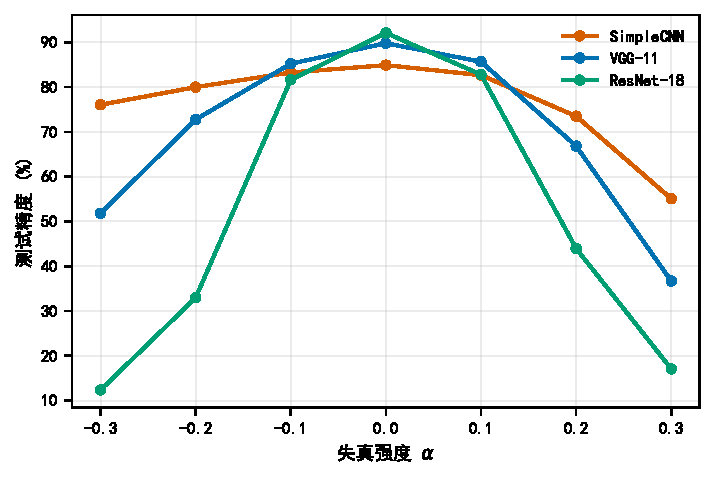
\includegraphics[width=0.68\textwidth]{C01_task1_sensitivity.pdf}
\caption{任务1：三个架构的非线性敏感性（CIFAR-10）。
$\alpha=+0.3$ 时 SimpleCNN / VGG-11 / ResNet-18 分别跌 29.82 / 53.10 / 75.01 个百分点。
数据：\texttt{outputs/task1\_*/alpha\_sensitivity.csv}。}
\label{fig:c01}
\end{figure}

\textbf{任务1}：正向失真的破坏力是负向的 3.4 倍（以 SimpleCNN 上 $|\alpha|=0.3$ 计）；
误差从浅层向深层累积，fc 层的输出与干净输出的余弦相似度仅 0.895；
残差连接是误差放大器——ResNet-18 的跌幅（75.01）远重于 VGG-11（53.10）与 SimpleCNN（29.82）。

\begin{table}[t]
\centering
\caption{任务2 与任务3 的关键读数（CIFAR-10，$\alpha=+0.3$，\%）}
\label{tab:phase12}
\small
\begin{tabular}{llccc}
\toprule
任务 & 配置 & SimpleCNN & VGG-11 & ResNet-18 \\
\midrule
\multirow{3}{*}{任务2}
& clean（基线） & 55.08 & 36.70 & 17.08 \\
& NAT-Scratch & \textbf{64.23}（$+9.15$） & \textbf{44.74}（$+8.04$） & 15.64（$\mathbf{-1.44}$） \\
& NAT-Finetune & 56.08（$+1.00$） & 39.96（$+3.26$） & \textbf{19.89}（$+2.81$） \\
\midrule
\multirow{3}{*}{任务3}
& Exp1（$+$残差校准） & 63.63 & --- & --- \\
& Exp2（$+$分层加权） & \textbf{68.76} & --- & --- \\
& Exp3（$+$非对称采样） & 69.14 & --- & --- \\
\bottomrule
\end{tabular}
\end{table}

\textbf{任务2}：非线性感知训练在纯前馈网络上有效（Scratch 策略 $+9.15$ / $+8.04$），
但残差网络在极限正向下失效甚至退化（$-1.44$）；效果与注入点数量负相关（5 $\to$ 9 $\to$ 18）。
中等失真上仍然有效（ResNet-18 在 $\alpha=-0.2$ 上 $+18.84$）。

\textbf{任务3}：叠加残差校准模块与分层加权采样后，SimpleCNN 的 $\alpha=+0.3$ 达 \textbf{68.76\%}。
消融显示分层加权是贡献最大的单项（$+5.13$），非对称采样边际贡献仅 $+0.38$；
三个配置的干净精度（87.19 / 87.37 / 87.59）全部高于未增强的干净模型（84.90）——
残差校准模块兼具正则化作用、不引入干净精度代价。

\begin{figure}[t]
\centering
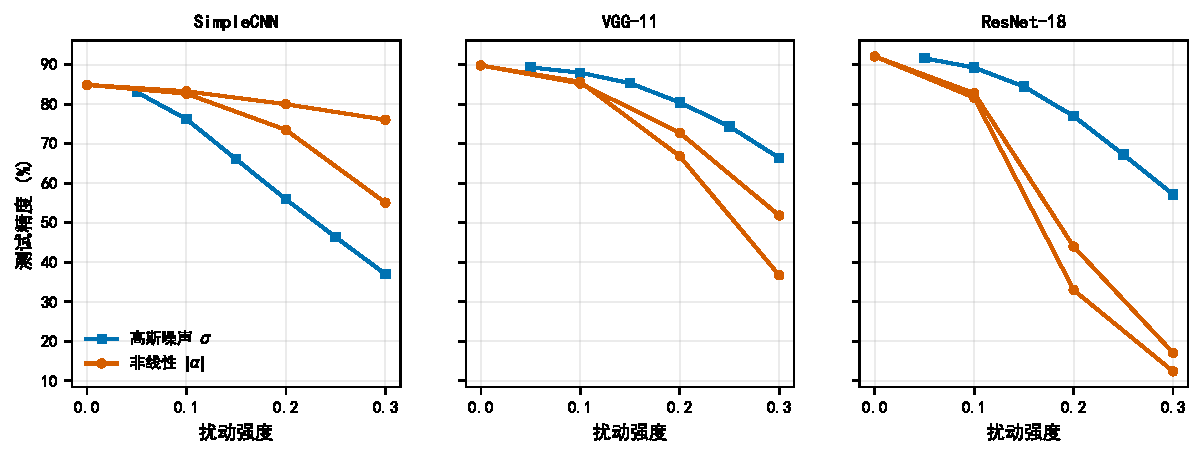
\includegraphics[width=0.92\textwidth]{C04_task_ext2_gauss_vs_nonlin.pdf}
\caption{拓展2：非线性失真与加性高斯噪声的对照（CIFAR-10）。
三种架构上的排序完全不同，ResNet-18 上两者完全反转。
数据：\texttt{outputs/extension2\_*/.../\{gaussian,nonlinearity\}\_sensitivity.csv}。}
\label{fig:c04}
\end{figure}

\textbf{拓展1--3}：脆弱性随深度与残差连接递增；
非线性失真与高斯噪声的鲁棒性\textbf{不可跨域迁移}（SimpleCNN 对高斯更脆弱 37.02 vs 55.08，
ResNet-18 则反之 57.15 vs 17.08）；
量化与非线性的联合作用呈\textbf{三分格局}——SimpleCNN 超加性恶化（4bit $\Delta=-7.23$）、
VGG-11 次加性即 Dithering（$\Delta=+7.82$）、ResNet-18 地板效应（$\Delta=+1.05$）。

\textbf{【第三阶段的细化：L3 两通路机制】}
上段"不可跨域迁移"在第三阶段被两步修订，此处补入归档（这是本项目最早确立的三条定律之一）。

\textbf{① 迁移层面——"零迁移"是架构依赖的。}
把一条通路训好的权重拿到另一条通路上扫，测扰动敏感性的变化幅度
$\max|\Delta_\sigma|$（>1.2 判非零）：SimpleCNN 1.16（Exp2 vs 原始）、
SimpleCNN 2.43（NAT vs clean）、\textbf{VGG-11 5.26（Exp2 vs clean，零迁移被打破）}、ResNet-18 1.41。
值得注意的是，给 SimpleCNN 加 3 个 MaxPool 反而把迁移\textbf{从 2.43 降到 0.98} ——
说明 MaxPool 密度不是迁移的成因。

\textbf{② 训练层面——不是零迁移，而是单向强干扰。}
同一 harness 上的 $2\times2$（是否注入 $\alpha$ $\times$ 是否注入 $\sigma$）：

\begin{center}
\small
\begin{tabular}{lcccc}
\toprule
训练条件 & clean & $\alpha=+0.3$ & $\sigma=0.30$ & 双扰动最坏点均值 \\
\midrule
无训练（clean 模型） & 59.99 & 28.09 & 3.98 & 16.04 \\
$\alpha$-only & 60.85 & 26.03 & 4.40 & 15.22 \\
$\sigma$-only & 55.79 & 22.01 & \textbf{27.19} & \textbf{24.60} \\
$\alpha+\sigma$（联合） & 55.20 & 15.27 & 31.31 & 23.29 \\
\bottomrule
\end{tabular}
\end{center}

$\alpha$ 训练对 $\sigma$ 几乎零收益（4.40 vs 3.98）；
但 $\sigma$ 训练使 $\alpha$ 侧从 28.09 掉到 22.01（$-6.08$，对 clean 模型），
联合训练进一步掉到 15.27（对只做 $\alpha$ 训练的 26.03 再低 $-10.76$）。
\textbf{双扰动并存时的最优配方是 $\sigma$-only，不是联合训练}——
joint 里的 $\alpha$ 注入是净负担（$\sigma$ 侧仅多拿 4.12，却付出 $\alpha$ 侧 $-10.76$）。
⇒ 正确表述是「\textbf{迁移近正交，但训练端存在单向强干扰}（$\sigma\to\alpha$ 有代价、$\alpha\to\sigma$ 无收益）」。

\textbf{数字出处}：上表三行取自 \texttt{outputs\_cifar100/v3\_methods/}
的 \texttt{gauss\_uniform} / \texttt{joint\_uniform} / \texttt{budget\_uniform} 三份
\texttt{alpha\_sensitivity.csv}（逐位可核）。迁移幅度表见第 \ref{sec:findings} 节
与 \texttt{论文v3.md} §8 勘误 12。

\begin{figure}[t]
\centering
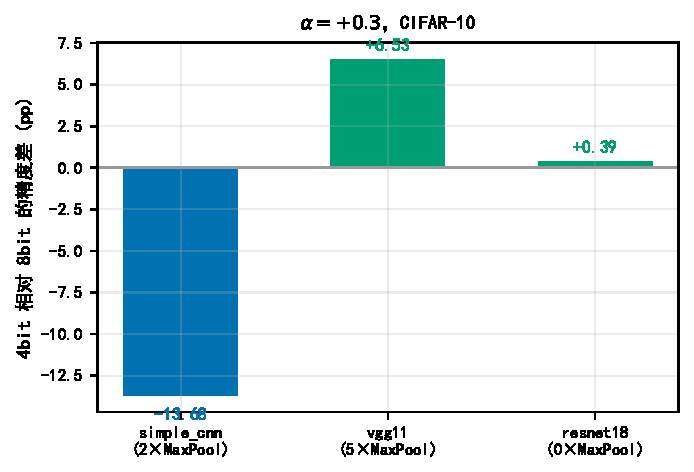
\includegraphics[width=0.62\textwidth]{C06_dithering_arch.pdf}
\caption{拓展3/优化二：Dithering 增益的架构依赖（CIFAR-10，$\alpha=+0.3$）。
增益与 MaxPool 密度同向，但要足够密——2 个 MaxPool 的 SimpleCNN 是负增益，
0 个的 ResNet-18 无效应。数据：\texttt{outputs/extension5\_dithering\_vgg11/arch\_dithering\_summary.csv}。}
\label{fig:c06}
\end{figure}

\textbf{优化二（Dithering 机理）}的关键结论在本节之后的"失真与量化的联合作用"中给出；
其核心是\textbf{否决了第一阶段给出的"随机共振"解释与"ADC 前注噪"建议}
（等剂量注噪的增益约为零），机理改写为"离散化分布重塑 $+$ MaxPool 架构载体"。

\begin{figure}[t]
\centering
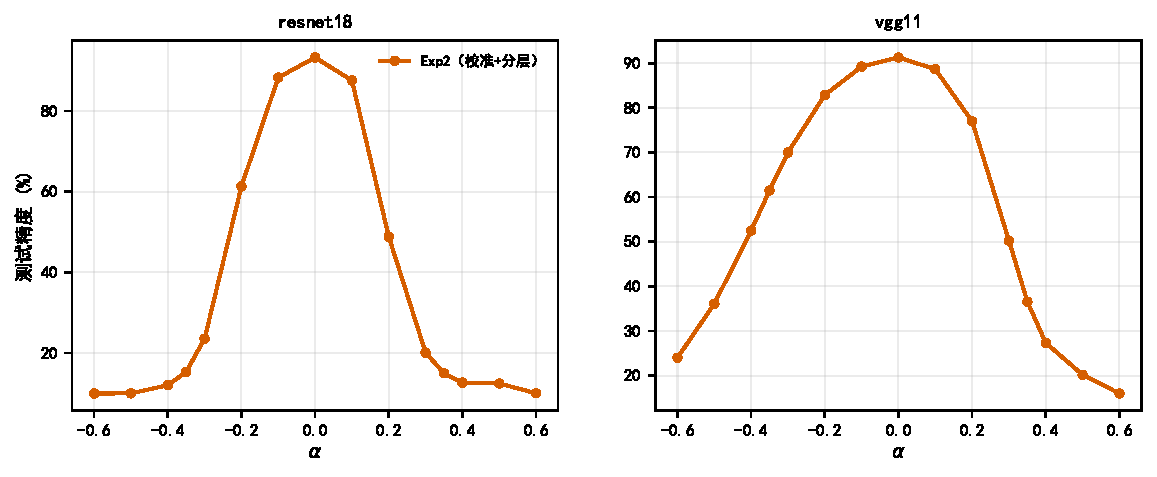
\includegraphics[width=0.88\textwidth]{C07_ext6_deep_transfer.pdf}
\caption{优化三：增强方案向深层主干迁移（CIFAR-10）。
灰色虚线为同架构干净模型，橙色为 Exp2 方案。
VGG-11 上 Exp2 在全部 15 个扫描点上都优于三条基线；
ResNet-18 上全程无败，但正侧强失真区的绝对精度仍然很低。
数据：\texttt{outputs/extension6\_deep\_robust/alpha\_wide\_scan\_deep\_robust.csv}。}
\label{fig:c07}
\end{figure}

\textbf{优化一（外推边界）与优化三（深层迁移）}的要点：
非线性感知训练的增益\textbf{严格限定在训练分布内}——
正侧在 $\alpha\approx0.4$ 处归零（$+0.77$）并反转为劣势（$\alpha=+0.5$ 时 $-10.77$），
而负侧随外推距离不降反升（$\alpha=-0.6$ 处 $+8.22$）；
架构容差窗口随深度单调收窄（SimpleCNN 约 $[-0.35,+0.25]$、
VGG-11 约 $[-0.25,+0.2]$、ResNet-18 约 $[-0.15,+0.15]$）。
Exp2 方案可完整迁移到深层：VGG-11 在 15 个扫描点上全胜三条基线（相对干净模型平均 $+10.22$），
ResNet-18 全程无败；$\alpha=+0.3$ 的增益为 $+13.55$ / $+3.04$；
两架构的干净精度（91.27 / 93.27）均为四组权重中最高。
多点校准（5/8 处）修复了 SimpleCNN 单点版本（1 处）在负侧外推输给 NAT-Scratch
最多 12.58 个百分点的短板。

\subsection{失真有多大破坏力，往哪里累积}

\begin{figure}[t]
\centering
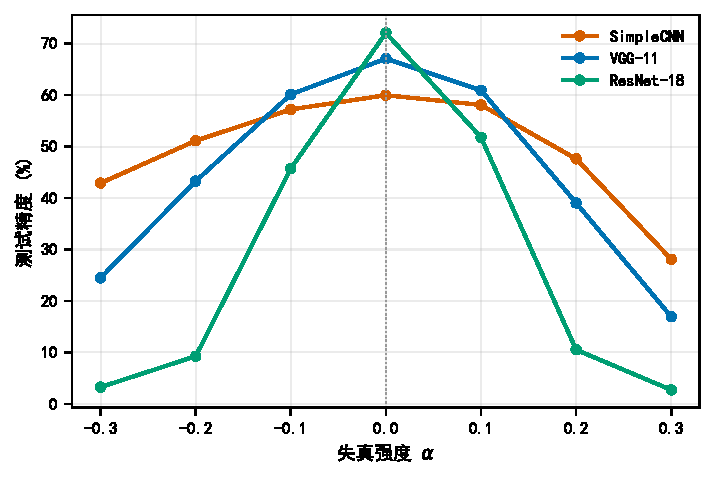
\includegraphics[width=0.70\textwidth]{F01_direction.pdf}
\caption{失真的方向性与容量依赖（CIFAR-100）。
三个主干在七点上的扫描；正侧跌落大于负侧（该方向在 SimpleCNN 与 VGG-11 上明显，
在 ResNet-18 上几乎消失：两侧跌幅 69.39 对 68.84），且随容量与深度单调放大。
数据：\texttt{outputs\_cifar100/task1\_*/alpha\_sensitivity.csv}。}
\label{fig:direction}
\end{figure}

$\alpha=+0.3$ 时 SimpleCNN 从 59.99 掉到 28.09、VGG-11 从 67.09 掉到 16.92、
ResNet-18 从 72.09 掉到 2.70。按容量排序，干净精度越高、跌幅越大，
这条反相关关系在同数据集内跨容量单调。

"3.4 倍不对称"这个常被引用的数字\textbf{不是常数}：
CIFAR-10/SimpleCNN/$|\alpha|=0.3$ 上是 3.4，CIFAR-100 同模型上只有 1.87。
它的适用域还很窄——CIFAR-100 的三个主干依次为 1.87 / 1.18 / 1.01，
CIFAR-10 的三个主干为 3.4 / 1.40 / \textbf{0.94}：
\textbf{方向随深度衰减，并在最深的主干上（CIFAR-10/ResNet-18）反号}。

把"最脆弱的位置"分成\textbf{注入位置}与\textbf{观测位置}后，一个反直觉结果出现：
单层注入探针中最敏感的是中间层卷积（conv2 跌幅 $-12.43$、conv3 $-7.56$），
而 fc 单点注入只有 $-0.68$。全 5 层同时注入的跌幅 31.90 远超线性累加的 23.33
（超加性 $-8.57$）。fc 是误差的\textbf{汇聚与观测点}，不是注入敏感点。

\subsection{灾难尾丢的不是信息，而是读出的可解码性}
\label{sec:mechanism}

这是全项目的枢纽结论。\cref{fig:probe} 用探针把它测出来。

\begin{figure}[t]
\centering
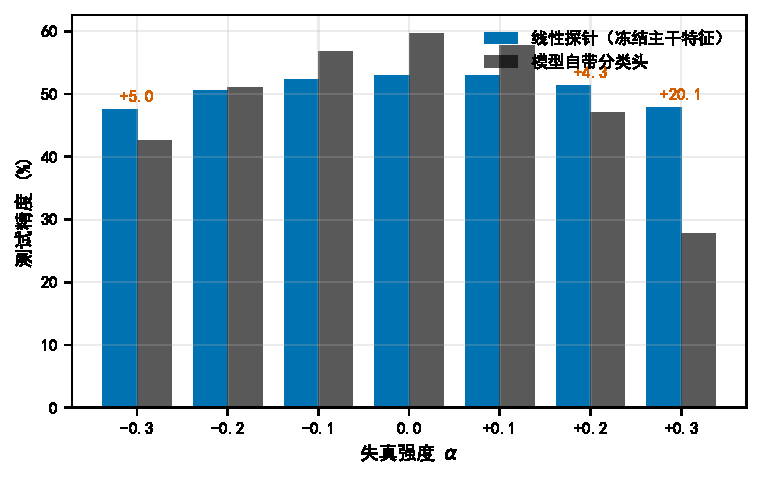
\includegraphics[width=0.76\textwidth]{F02_probe_headroom.pdf}
\caption{探针 headroom：灾难尾的标签信息仍然线性可达。
在同一冻结主干的末端特征上，线性探针（实心）与\textbf{原始头}
（空心，即模型自带的分类头，产物里的 \texttt{a\_original\_fc}）的精度；
7 个 $\alpha$ 点，CIFAR-100 \textbf{全量测试集}（10\,000 张）、best 权重、单种子。
$\alpha=+0.3$ 时相差 20.26 个百分点；同样的探针在加性高斯噪声 $\sigma=0.3$ 下只有 7.50。
数据：\texttt{outputs\_cifar100/v7\_probe\_audit/ra\_onprotocol\_main.csv}。}
\label{fig:probe}
\end{figure}

$\alpha=+0.3$ 时探针达 48.35\%、原始头 28.09\%，headroom \textbf{20.26}%
\footnote{两项均取自\textbf{全量测试集}（10\,000 张），与项目的规范口径逐位一致
（$\alpha=+0.3$ 的 28.09 等于 \texttt{task1} 同名行；$\alpha=0$ 的 59.99 等于 \texttt{metrics.json}
的 \texttt{best\_test\_acc}）。早期版本曾用 8000 样本子集，给出 27.76 / 59.60 与 $+20.12$；
第七阶段 M0c 已在同一设备（CUDA）上重跑全量口径并替换，全案见 \texttt{docs/IMPL\_AUDIT.md}
与台账 \S16.0。}；
$\alpha=+0.4$ 时 30.90、$+0.5$ 时 30.82。headroom 随失真增强先放大、后趋于平坦
（$+0.3\to+0.4$ 增幅最大，$+0.4\to+0.5$ 微降 0.08——不是单调上升）。

\textbf{口径标注（必读）}：该探针\textbf{逐 $\alpha$ 条件训练}——它在每个测试点的失真特征上
重新拟合线性头（源文件 \texttt{ra\_onprotocol\_main.csv} 的 \texttt{probe\_same\_cond} 列，
与之并列的 \texttt{probe\_clean\_train} 列则只在干净特征上训练）。
因此 headroom 是 \textbf{oracle-$\alpha$} 诊断量：它回答的是"若已知失真强度、且读出可自由重训，
线性解码还能恢复多少"，\textbf{不是可部署读数}——不知道 $\alpha$ 时的实际读出读数是 43.31
（见第 \ref{sec:findings} 节的读出适配）。作为对照，只在干净特征上训练的探针在
$\alpha=+0.3$ 上只有 18.1，低于原始头（28.09）。

\textbf{对照通路的判别力}：同一套探针在加性高斯噪声 $\sigma=0.3$ 下 headroom 只有 7.50。
随机扰动与确定性系统误差在"信息还剩多少"这个量上清楚地分开。

\subsection{修复：冻结主干、只重训线性读出}

\begin{figure}[t]
\centering
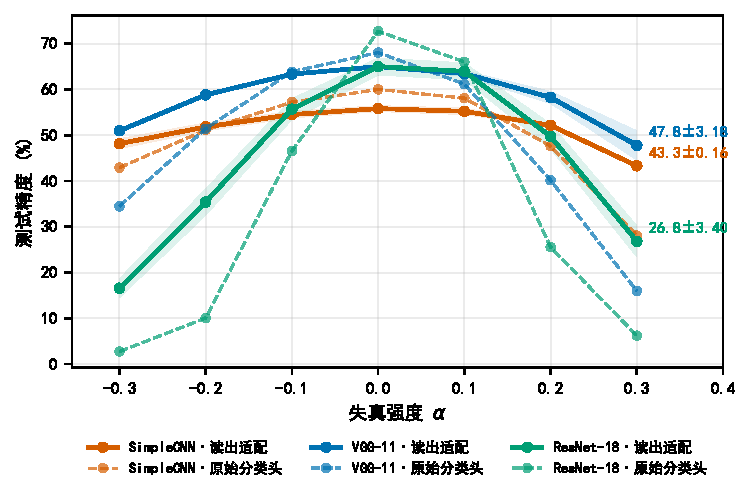
\includegraphics[width=0.74\textwidth]{F03_readout_nat.pdf}
\caption{读出适配跨三个主干一致抬升尾部（CIFAR-100，3 个种子的逐点均值）。
实线为\textbf{读出适配}（readout-NAT，主干全冻结，可训练参数占全模型 5.04\%/0.55\%），
虚线为各模型的原始头。
数据：\texttt{outputs\_cifar100/v3\_readout\_repair/*ep24*.csv}。}
\label{fig:readoutnat}
\end{figure}

\begin{table}[t]
\centering
\caption{读出适配 vs 全网络鲁棒训练（CIFAR-100，$\alpha=+0.3$，精度 \%）}
\label{tab:nat}
\small
\begin{tabular}{lcccc}
\toprule
方法 & 训练成本 & SimpleCNN & VGG-11 & ResNet-18 \\
\midrule
原始头（同主干） & --- & 28.09 & 15.98 & 6.22 \\
\textbf{读出适配（24ep，3 seed）} & \textbf{12$\sim$30 min} & \textbf{43.31}$\pm$0.16 & \textbf{47.79}$\pm$3.18 & \textbf{26.82}$\pm$3.40 \\
全网络鲁棒训练（最好） & 1$\sim$6.5 h & 29.89 & 24.69 & 6.22 \\
\bottomrule
\end{tabular}

\vspace{3pt}
\begin{minipage}{0.94\textwidth}
\footnotesize
\textbf{表注（口径）}：\textbf{第一行}为各读出实验所依附主干的\textbf{原始头}
（\texttt{v3\_readout\_repair} 的 \texttt{a\_original\_fc} 行在 $\alpha=+0.3$ 的读数；
SimpleCNN 的该主干即 \texttt{task1} 权重，故与台账逐位一致）。
\textbf{第三行}为各架构上最好的全网络鲁棒训练配方（SimpleCNN 取该主干在全网络下的最优结果
\textbf{29.89}；\textbf{同协议 3 seed 的 v3 路径逐层独立 NAT 均值是 26.57，低于 29.89，故本行取 29.89}；
VGG-11 与 ResNet-18 取 200\,ep 的 Exp3，24.69 / 6.22）。
注意 \textbf{ResNet-18 的第三行与该列第一行是同一块主干}——全网络配方并没有改善它的原始头。
（\texttt{task1} 主干的 16.92 / 2.70 属另一批权重，不参与本表逐列比较。）
\end{minipage}
\end{table}

读出适配在三个主干上一致超过"全网络重训"整类配方，可训练参数只占 5.04\%/0.55\%，
训练成本\textbf{逐主干配对}为 1/5、1/16、1/13（读出 12 / 25 / 30 min 对全网络 1 / 6.5 / 6.5 h），
约低一个数量级。
代价是干净精度下降 3.08$\sim$7.69 个百分点（$\alpha=0$ 处：读出适配的三 seed 均值为
55.81 / 64.97 / 65.00，对各自主干的原始头 59.99 / 68.05 / 72.69）。

\textbf{必要的自我校验}：单点读出适配（只对 $\alpha=+0.3$ 拟合）确实是再分配——
该点 $+24.70$ 但干净精度 $-20.36$、$\alpha=-0.3$ 掉 25.71，七点均值反而低于基线。
起作用的是\textbf{分布式}版本（$\alpha\sim U[\pm0.3]$ 上训练），它在每个扫描点都不显著劣化。
同一层参数、两种训练方式给出质上不同的结果。

\textbf{这条结论不只有探针读数背书}：冻结主干、只重训一个线性头，
在 $\alpha=+0.3$ 上\textbf{实际达到 43.31}（SimpleCNN，3 seed，24\,ep 协议；同期原始头 28.09）——
那是一个\textbf{真实可部署的分类器}，不是仅用于测量的探针。
同口径的 \textbf{oracle-$\alpha$} 探针读数为 48.35，即部署物取到了上界的 \textbf{89.6\%}
（$43.31/48.35$）。注意分母是 \textbf{oracle-$\alpha$} 口径（假定失真强度已知），
因此这个比例\textbf{不是}"部署时可以达到 89.6\%"的意思。

\subsection{训练端的四条路径为什么都没能改善尾部}

\begin{figure}[t]
\centering
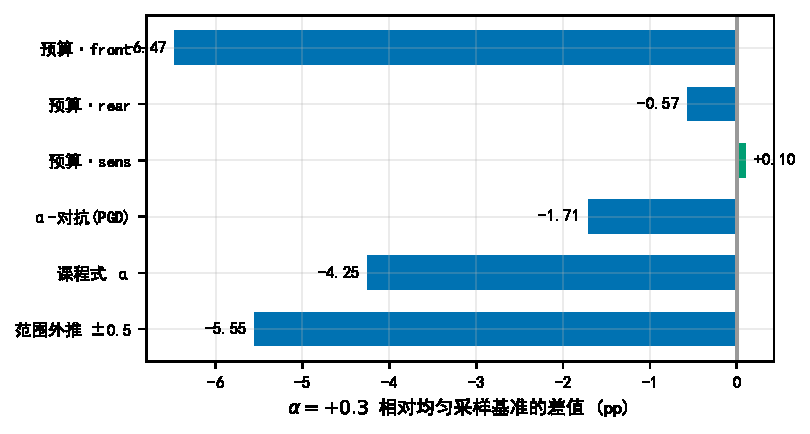
\includegraphics[width=0.68\textwidth]{F04_training_paths.pdf}
\caption{训练端的补救路径在 $\alpha=+0.3$ 上没有一条\textbf{显著}优于均匀采样基准（CIFAR-100 / SimpleCNN）。
数据：\texttt{outputs\_cifar100/v3\_methods/*/alpha\_sensitivity.csv}。}
\label{fig:training}
\end{figure}

四条独立路径：采样预算分配（三种轮廓，最好 26.13，$+0.10$）、$\alpha$ 空间对抗训练（24.32，$-1.71$）、
课程式采样（21.78，$-4.25$）、训练范围外推至 $\pm0.5$（20.48，$-5.55$）。
基准（均匀采样）为 26.03。按本文自订的单种子门槛
（尾部差值小于 3 个百分点不作为结论），其中只有课程式与外推两条可记为显著劣于基准
（$-4.25$ / $-5.55$），对抗训练的 $-1.71$ 落在门槛内、记为\textbf{不可分辨}，
预算分配的 $+0.10$ 与基准同级。\textbf{四条都没有改善尾部。}

最强的一条证据是范围外推：\textbf{模型已在 $\pm0.5$ 上训练过}，
测试 $\alpha=+0.5$ 时仍只有 2.71\%，同期负侧 $-0.5$ 有 31.19\%（差 28.5 个百分点）。
正侧尾部不是采样覆盖问题，而是\textbf{结构性的不可训练区}。

\subsection{损伤的形态：维度丢失，不是类间距缩小}

\begin{figure}[t]
\centering
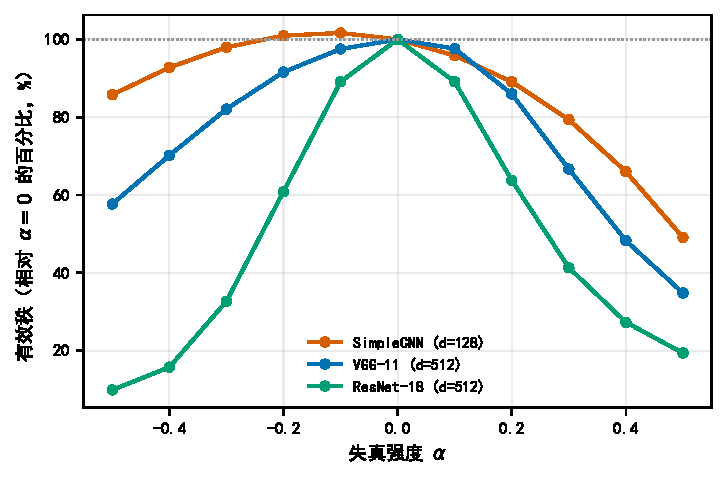
\includegraphics[width=0.68\textwidth]{F05_rank_collapse.pdf}
\caption{正侧失真使末端特征的有效秩塌陷；负侧的形态随主干而异
（SimpleCNN 几乎不动，VGG-11 与 ResNet-18 两侧都塌，ResNet-18 的负侧更甚）。
纵轴为按各模型 $\alpha=0$ 归一化的有效秩 $\exp(-\sum p_i\ln p_i)$；
特征维数分别为 128 / 512 / 512。
数据：\texttt{outputs\_cifar100/v5\_rank\_collapse/rank\_stats*.csv}。}
\label{fig:rank}
\end{figure}

$\alpha=+0.3$ 时有效秩下降 20.6\% / 33.3\% / 58.7\%（三个主干）；
负侧同强度下降 \textbf{2.0\% / 17.9\% / 67.3\%}——
\textbf{"负侧几乎不动"只在浅层的 SimpleCNN 上成立}，
而 \textbf{ResNet-18 的负侧（67.3\%）比正侧（58.7\%）掉得更多}，
其 $+0.3$ 与 $-0.3$ 精度也同样是两侧都崩（2.70 / 3.25）。
⇒ \textbf{秩塌陷解释"正侧特殊"这条链，只在秩塌陷本身不对称的主干上才连得起来。}

关键在于\textbf{浅层主干上}：\textbf{同强度下正侧的 Fisher 判别比反而高于负侧}——
类间可分性没有变差，丢失的是\textbf{维度}。
这与幅度统计一致：$\alpha>0$ 把深层特征的幅度向中段压缩
（fc 与 conv1 的 L2 范数比从 0.45 降到 0.23），端点不变而中段被压低。

这解释了"信息还在但训练救不回"的表面矛盾：信息仍存在于剩余维度里，
但这些维度在主干参数的可达域之外。

\begin{figure}[t]
\centering
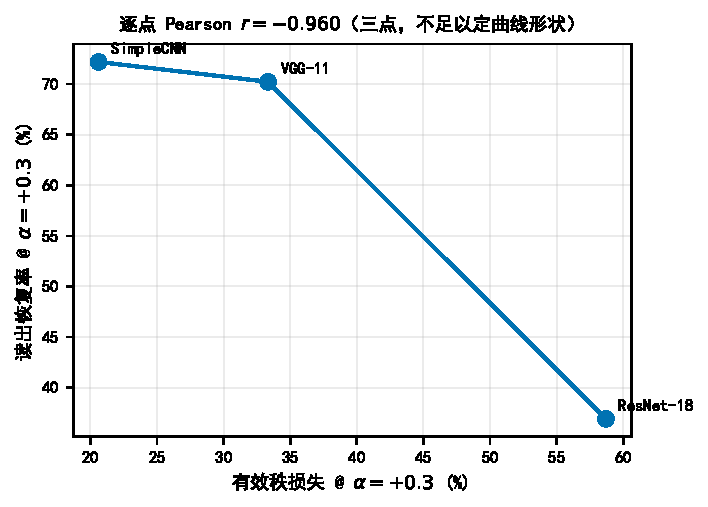
\includegraphics[width=0.56\textwidth]{F06_rank_vs_recovery.pdf}
\caption{秩损失与读出可恢复量（三点，$r=-0.960$）。
恢复率 = 读出适配 @$\alpha=+0.3$ 的精度 $\div$ 同一文件里原始头 @$\alpha=0$ 的精度。
\textbf{三点不足以定曲线形状}；形状提示为"先平后塌"。}
\label{fig:rankrec}
\end{figure}

\subsection{第二个杠杆：池化密度}

\begin{figure}[t]
\centering
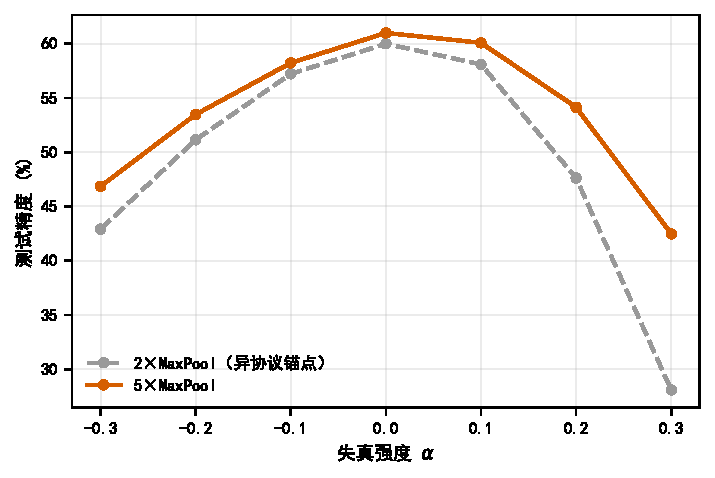
\includegraphics[width=0.68\textwidth]{F07_maxpool_density.pdf}
\caption{池化密度是零训练成本的独立架构杠杆。
MaxPool 从 2 个加到 5 个（参数量不变、训练脚本不变）：
$\alpha=+0.3$ 从 28.09 到 42.47。虚线为\textbf{第一阶段脚本}的产物：
它与实线出自\textbf{不同训练脚本}（本项目实测跨脚本的精度数字不可直接比较），
故属异协议、仅作锚点，不与实线并列比较。}
\label{fig:maxpool}
\end{figure}

5 个 MaxPool 的那一支以下简称\textbf{mp 主干}（表 \ref{tab:arch} 的 SimpleCNN+3$\times$MaxPool）。
$\alpha=+0.3$ 从 28.09 提升到 42.47（干净训练）、26.03 到 41.55（鲁棒训练；
两侧同为逐层独立采样，同 seed 配对，增益 $+15.52$），
七点均值提升 4.5$\sim$4.9 个百分点，干净精度不降。

\textbf{机制：保护主要来自降维。} 三个候选解释被逐一排除：

\begin{table}[t]
\centering
\caption{池化保护的三个候选解释与排除依据}
\label{tab:pool}
\small
\begin{tabular}{p{2.6cm}p{4.2cm}p{6.6cm}}
\toprule
候选解释 & 检验 & 结论 \\
\midrule
池化"吸收"了失真 & 归一化三次映射与 max 是否可交换
& 在池化输入（post-ReLU，非负）上\textbf{精确可交换}（$\max|\Delta|=0.000\text{e}{+}00$），
  但可交换却非成因 \\[2pt]
质量向恒等区集中 & 5-pool 与 2-pool 的易感度 $S$ 与不变区占比
& 5-pool 的 $S$ \textbf{反而更高}（conv4：0.1527 vs 0.1134），不变区占比不变 \\[2pt]
max 的选择性 & 换成 top-2 池化（与 $f_\alpha$ 不可交换）
& 保护与 max 等同（42.98 vs 42.47，单种子） \\
\bottomrule
\end{tabular}
\end{table}

三条排除后，唯一显著差异是\textbf{空间元素数从 256 降到 16}。
同协议 3 种子对照：5$\times$max 的 \texttt{drop@0.3} 为 $20.60\pm1.54$、
5$\times$avg 为 $21.78\pm0.91$，差 $+1.17$（标准误 1.03，$z\approx1.1$）→
\textbf{"降维 : 非均值聚合"的定量比例不予裁决}，只给方向：\textbf{保护主要来自降维}。

\subsection{两个杠杆的叠加与在线估计}

架构杠杆与读出杠杆在尾部\textbf{可以同时受益，但显著次可加、不是相加}：
\texttt{mp 主干 $+$ 读出适配} 的 $\alpha=+0.3$ 达 \textbf{49.12}
（相对基线 28.09 即 $+21.03$），而两个手段单独的增益之和是 $+29.67$
（架构 $+14.38$ 与读出 $+15.29$ 分别取自同批\textbf{单 seed} 产物的 42.47 与 43.38）
——\textbf{合起来只拿到六到七成，损失三到四成}。
本段四个数（28.09 / 42.47 / 43.38 / 49.12）\textbf{全部为单 seed 口径}
（连续均匀 $\alpha$、24\,ep、20k 样本，同 v3 路径）；
13 点离散 $\alpha$、3 seed 的 v5 口径给出同样的次可加结论。

失真强度可由读出特征的岭回归在线恢复：四个主干$\times$数据集组合上
$R^2$ \textbf{0.827$\sim$0.935}、MAE \textbf{0.036$\sim$0.061}。

\subsection{门控的边界}

\begin{figure}[t]
\centering
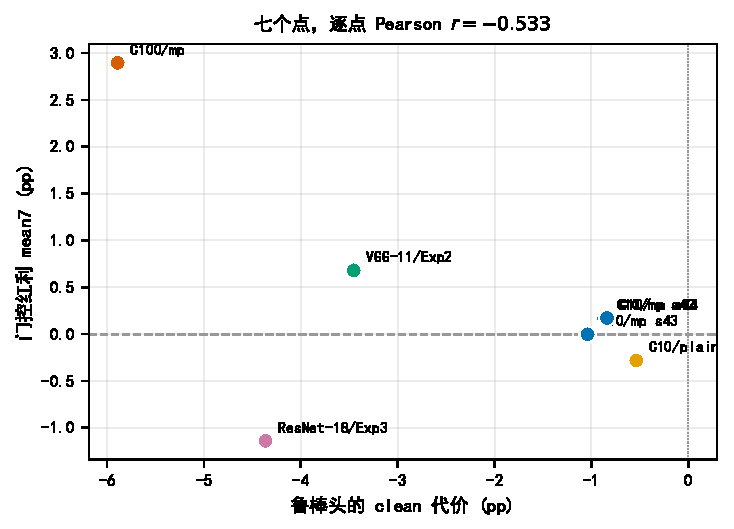
\includegraphics[width=0.68\textwidth]{F08_gating_benefit.pdf}
\caption{门控红利不随鲁棒头代价单调增长。
七个点取自四个主干配置与两个数据集，各 3 个种子。
七点 $r=-0.533$；去掉 CIFAR-100 远点后 $n=6$ 时符号反转为 $+0.351$。
数据：\texttt{v5\_full\_recipe/recipe*.csv}。}
\label{fig:gating}
\end{figure}

CIFAR-100 的 mp 主干上，\textbf{鲁棒头}（即读出适配头，此处沿用产物列名
\texttt{acc\_robust\_head}）的干净代价 $-5.89$、门控收回 $+2.90$；
但把深层主干加进来后，代价落进此前空白的 2$\sim$5 个百分点区间
（VGG-11 $-3.45$、ResNet-18 $-4.36$），\textbf{红利却没有跟着变大}
（$+0.68$ 与 $\mathbf{-1.14}$）。

原因：ResNet-18 的原始头在负侧是崩的（$\alpha=-0.2$ 只有 10.27\%）。
软门控按 $w=|\hat{\alpha}|/0.3$ 插值，在 $\alpha=-0.2$ 处 $w\approx0.67$，
三分之一权重的坏头把 45.64 拖到 39.21。

\textbf{门控有效需要两个前提同时成立}：① 鲁棒头干净代价足够大；② 两个头在整个 $\alpha$ 轴上都不能崩。
两前提\textbf{无法}做成装前的量化自检——两种候选定义在已有 7 个点上都不分离红利的符号
（VGG-11 的最小精度只有 15.73 却红利为正；CIFAR-10 的 mp 主干（主干种子 43）
的最小精度有 69.23 却红利为 $-0.003$）。

\subsection{失真与量化的联合作用}

\begin{figure}[t]
\centering
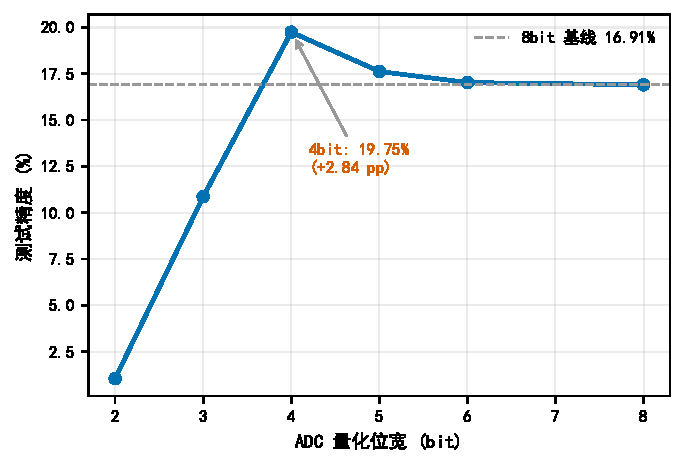
\includegraphics[width=0.60\textwidth]{F10_dithering.pdf}
\caption{低位量化在池化密集架构上反转成增益（VGG-11，$\alpha=+0.3$，CIFAR-100）。
4bit 时精度最高，比 8bit 高 2.84 个百分点。
数据：\texttt{outputs\_cifar100/extension5\_dithering\_vgg11/group\_a\_bits\_scan.csv}。}
\label{fig:dithering}
\end{figure}

VGG-11 上 4bit 量化的精度\textbf{高于} 8bit（CIFAR-100 $+2.84$、CIFAR-10 $+6.53$）。
三假设判决（\textbf{以下机理数字全部取自 CIFAR-10 侧}的
\texttt{outputs/extension5\_dithering\_vgg11/}——该目录才是当时跑机理分析的完整批量；
CIFAR-100 侧的对应量见段末）：\textbf{H1 随机去相关否决}（等剂量注噪 $-2.45/-1.87$，
8bit$+$最优剂量噪声 $-0.03$；样本级翻转 4bit 为 4.15:1 而噪声条件约 1:1）、
\textbf{H2 分布重塑确认}（分类器输入峰度 1.486 $\to$ 0.110，4bit 恢复到 0.214）、
\textbf{H3 MaxPool 交互支持（必要条件）}（无 MaxPool 的 ResNet-18 免疫 $+0.39$，
但 2 个 MaxPool 的 SimpleCNN 是 $-13.68$）。

\textbf{CIFAR-100 侧的平行读数}（同批统计，见
\texttt{outputs\_cifar100/extension5\_dithering\_vgg11/}）：峰度 2.541 $\to$ 0.847，
4bit 恢复到 0.980；翻转 4bit 为 655:371（1.77:1），噪声条件同样接近 1:1；
ResNet-18 的 4bit 减 8bit 增益为 $-0.21$、SimpleCNN 为 $-14.71$。
\textbf{三条判决在两个数据集上同向}（H2 的"峰度恢复"在 CIFAR-100 上幅度较小），
这本身是一条跨数据集稳健性证据。

\section{研究历程：三次"先归因、后被自己否证"}
\label{sec:history}

本节记录本项目最贵的一课。三次的形态完全一样：
一个被当成"噪声"或"实现细节"的差异，被重新命名成一个"效应"，
又被实验否证，最后回到未知。

\subsection{第一次：把处理效应误读成噪声（$\pm3.15$ 混协议）}

\textbf{当时的判断}：一组鲁棒训练的 3 个种子，$\alpha=+0.3$ 的读数是 21.41 / 26.73 / 26.95，
标准差记为"尾部种子噪声 $\pm3.15$ 个百分点"（同期干净精度只有 $\pm0.51$）。
据此立下全项目规则：涉及尾部指标的对比必须 $\ge3$ 个种子，单种子尾部差值 $<3$ 个百分点不构成结论。

\textbf{问题}：这 3 个种子来自\textbf{两个脚本}。

\textbf{否证}：补跑同脚本的第三个种子后，同协议的尾部标准差只有 $\pm0.392$，
而混协议组是 $\pm2.561$——\textbf{方差被估高约 6 倍}。
进一步的定量分解显示：混合组里两个数相差 5.32，与实测的脚本级处理效应 5.52 几乎相等，
也就是说 \textbf{那 2.56 里绝大部分不是随机噪声，而是两种训练配方之间的系统差}。

\textbf{制度补丁}：\textbf{方差对比必须同脚本、同一采样代码路径}。

\subsection{第二次：把脚本差异误读成采样粒度}

\textbf{当时的判断}：同 seed 下两个脚本的 $\alpha=+0.3$ 相差 4.62 个百分点，
是纯协议标准差的约 11.8 倍。两脚本在数据加载、归一化、优化器、batch、epoch、调度器、
增强、钩子机制、采样位置与评估口径上\emph{逐项核对一致}，
因此判定"目前唯一可辨识的实现差异就是 $\alpha$ 采样粒度（每批共享 vs 逐层独立）"，
并把它提升为候选定律。

\textbf{否证}：在\textbf{同一个脚本里只切换粒度}：
shared 26.55 vs per-layer 26.57，差 $+0.02$（$z=0.08$）；
而\textbf{同粒度跨脚本}差 $+5.52$（$z=9.4$）。
\textbf{效应跟着脚本走，不跟着粒度走。}

\textbf{制度补丁}：涉及跨脚本比较时，\textbf{先做一次交叉评估}
（把 A 的权重量到 B 的评估路径下），确认评估侧无差。
这条制度立刻在下一个实验中产生了价值。

\textbf{更深的教训}：\textbf{"逐项排除混杂"这种论证在跨实现比较里不成立。}
两脚本的 8 项都一致、训练损失逐 epoch 差 $\le0.016$，效应却稳定存在。
\textbf{没查出差异 $\ne$ 没有差异。}

\subsection{第三次：把序列位置误读成消耗数}

\textbf{当时的判断}：交叉评估把差异锁到"权重侧"（见下），
再据 $\alpha$ 采样轨迹把根因定为"随机数流错开"——
一个脚本的 shared 模式消耗 5 个随机数、另一个只消耗 1 个，
第 1 个 batch 相同、之后完全错开。

\textbf{否证}：在\textbf{同一个脚本里}把消耗数从 5 改成 1：26.66 vs 26.55，差 $+0.11$。
\textbf{消耗数不是因果。}

\begin{figure}[t]
\centering
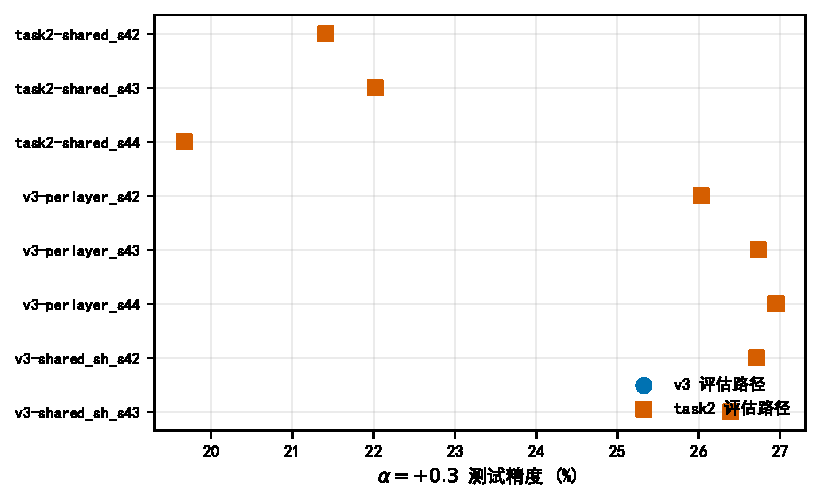
\includegraphics[width=0.70\textwidth]{F09_crosspath.pdf}
\caption{交叉评估：差异不在评估路径。
8 个权重分别在另一脚本原样导入的评估函数下重扫，两条路径给出\textbf{逐位相同}的读数；
但两组权重稳定分成两簇。
数据：\texttt{outputs\_cifar100/v6\_p4e\_crosspath/crosspath.csv}。}
\label{fig:crosspath}
\end{figure}

\begin{table}[t]
\centering
\caption{5.55 个百分点差异的三次归因尝试}
\label{tab:mystery}
\small
\begin{tabular}{p{2.2cm}p{3.4cm}p{8.6cm}}
\toprule
轮次 & 归因 & 结果 \\
\midrule
1 & 尾部\textbf{种子噪声} $\pm3.1$
& 否证：三种子来自两脚本；同协议标准差只有 $\pm0.39$，混协议把方差估高约 6 倍 \\[2pt]
2 & $\alpha$ 采样\textbf{粒度}
& 否证：同脚本切换粒度差 $+0.02$（$z=0.08$），同粒度跨脚本差 $+5.52$（$z=9.4$） \\[2pt]
3 & 随机数\textbf{消耗位置}
& 否证：同脚本把消耗数从 5 改成 1，差 $+0.11$ \\
\bottomrule
\end{tabular}
\end{table}

\textbf{最终图景}：一个脚本训出的鲁棒权重稳定落在 $\mathbf{21.03\pm1.00}$（3 个种子，
逐 seed 19.67$\sim$22.02），另一个脚本的\textbf{六个} run 全部落在 $\mathbf{26.58\pm0.29}$
（逐 run 26.03$\sim$26.95），两组相差 \textbf{5.55} 个百分点（$z=9.4$）。
\textbf{组内极紧、组间稳定分离}——这正是最令人困惑的地方：
同脚本内换种子的流差异只值 $\pm1$，跨脚本却稳定值 5.55。

\textbf{已排除的解释累计}：种子噪声、$\alpha$ 采样粒度、随机数消耗数、
评估路径（8 个权重 $\times$ 2 条路径逐位相同）、训练动力学（逐 epoch 损失差 $\le0.016$）。
\textbf{仍未归因，按已知未知记录。}

\textbf{最终的结论（限定形式）}：\textbf{本文观测到一个同超参、同种子、跨实现稳定
5.55 个百分点的差异，经三次干预实验仍未归因}。在归因之前，\textbf{我们的做法是}
不跨实现引用精度数字，部署校准与部署训练保持同实现、同路径。
\textbf{这不排除"某一脚本里还有一个尚未找到的具体差别"}——把一个未定位的差异
直接命名为"实现层普遍不可移植"，证据不足。

\subsection{三次翻案的共同点与制度沉淀}

三次都是\textbf{用自己的实验推翻自己上一轮的结论}。
三次的根因按项目内部的总结都是"\textbf{没做交叉评估}"——
或者说，\textbf{在跨实现的比较里，任何没有做干预实验的归因都只是命名，不是因果}。

沉淀下来的三条制度：

\begin{enumerate}[leftmargin=2em,itemsep=2pt]
  \item \textbf{降级一个数字，必须扫它的整条引用链}。
        含均值、差值、占比这些\textbf{派生量}——它们不带原值，模糊搜索抓不到。
        这条制度立起来的原因是：一次降级只改了被降级的那一节本身，
        而它派生出去的数字还在下游活着（其中一处甚至是"同一行内混了两个脚本"）。
  \item \textbf{方差对比三要求}：同脚本 / 已交叉评估 / 未校准的组必须标注。
        后续补充第四条：跨实现比较前先做消耗数等价检查；
        且"同脚本 $+$ 交叉评估"\textbf{不足以}让两套跨脚本数字可比。
  \item \textbf{判据跑前写死，跑后不改}。六个阶段的每个实验都在台账里留了预登记，
        包括那些最终被否证的。
\end{enumerate}

\section{第七阶段：归档后的自主迭代}
\label{sec:v7}

\begin{quote}
\small 归档（tag \texttt{v1.0-archive}）之后又进行了一轮自主迭代。
本节记录它的产出——分两类：\textbf{加强结论的}，与\textbf{排除解释的}。
详细台账见 \texttt{experiments\_ledger.md} §16。
\end{quote}

\subsection{两条加强中心结论的结果}

\textbf{(1) 容量不是这里的瓶颈。}
此前所有读出都是\textbf{线性}的，所以"瓶颈在读出"有一个明显的反驳：
也许瓶颈只是在线性。为排除它，在同一批冻结特征上比较六种读出
（$\alpha=+0.3$，CIFAR-100，$n_{\text{train}}=8000$）：

\begin{center}
\small
\begin{tabular}{lc}
\toprule
读出 & 精度（\%） \\
\midrule
\textbf{线性头（torch，同族公平锚）} & \textbf{51.47} \\
强正则逻辑回归（$C=0.01$） & 49.23 \\
sklearn 逻辑回归（跨优化器参考臂） & 48.25 \\
两层 MLP（$128\to256\to100$） & 48.62 \\
瓶颈 MLP（$128\to32\to100$） & 43.38 \\
k-NN（$k=20$） & 38.12 \\
\bottomrule
\end{tabular}
\end{center}

三种非线性读出\textbf{没有一个超过线性头}（相对线性头 51.47：k-NN 38.12 即 $-13.35$、
瓶颈 MLP 43.38 即 $-8.09$、两层 MLP 48.62 即 $-2.85$）。
前两者的差距远超本轮立的可分辨门槛（$\Delta_{\text{proc}}=3.45$ pp，见下）；
\textbf{两层 MLP 只差 2.85，落在门槛内、按本文自订规则不可裁决}，方向上仍劣于线性头。
而且\textbf{参数越多反而越差}——典型过拟合序。⇒ 「信息仍线性可达」从"只测过线性"升级为
「\textbf{测过 k-NN 与两种 MLP 之后，线性头仍是最优读出}」。

\textbf{(2) headroom 是下界，而且可以抬高。}
把探针的训练样本从 8000 加到 50000（训练集全量）：

\begin{center}
\small
\begin{tabular}{lccc}
\toprule
& 探针（$n$=8000） & 探针（$n$=50000） & 冻结头 \\
\midrule
clean & 53.56 & \textbf{59.00} & 59.99 \\
$\alpha=+0.3$ & 48.35 & \textbf{55.72} & 28.09 \\
\midrule
headroom @$+0.3$ & $+20.26$ & $\bm{+27.63}$ & --- \\
\bottomrule
\end{tabular}
\end{center}

\textbf{且仍未饱和}（等宽对数斜率比 $r=0.96/0.61$，判据要求 $\le0.5$）。
按"不相交划分"校正后约 $+25.4$（$=27.63-2.19$；其中 2.19 pp 是"探针训练集与主干训练集
\textbf{不相交}"这一口径在 $\alpha=+0.3$ 上比分布内低的量，出自台账 \S16.0a 的三臂对照，
此处按同口径移用到 $n$=50000 档）。

\textbf{这条观测的含义比数字本身重要}：$+20.26$ 不是表征的某个固定属性，
它是"探针只喂了 8000 个样本"下的读数。
⇒ \textbf{headroom 是读出训练方式的函数}——与下面那条"过程自由度"是同一件事的两个侧面。
\textbf{读出这一层不是免费的。}

\subsection{四条排除型结论}

\begin{center}
\small
\begin{tabular}{p{4.2cm}p{9.6cm}}
\toprule
方向 & 判决 \\
\midrule
ETF / 原型读出 & \textbf{无增益}。三种原型或 ETF 正则读出均未超过线性头，
  且几何诊断（下一条）事先预测了这一点 \\
神经坍缩（NC）几何 & \textbf{远离 ETF}。类均值夹角偏离与模长变异系数在正侧 5/5 上升
  ⇒ 「正侧 Fisher 反而高于负侧」这条异常\textbf{不能用 NC 解释} \\
"少样本即可恢复全表示" & \textbf{不成立}。读出样本量曲线在 500$\sim$50000 上单调上升且\textbf{未饱和}，
  需数千量级样本 \\
门控两前提的装前自检 & \textbf{不分离}。两种候选量化定义在已有的 7 个点上都分不开红利的符号 \\
\bottomrule
\end{tabular}
\end{center}

\textbf{排除型结论的价值在于：它们各自堵死一个替代解释。}
尤其第一条——原来"读出瓶颈"可以被反驳为"你只测了线性头"，现在这个反驳不成立了。

\subsection{方法学产出（本阶段最值钱的部分）}

\textbf{(a) 三级可分辨性。}
「跨实现不可移植」是一个已知未知，无法直接当门槛用。但它旁边两级\textbf{可测}的散布，
合起来给出一个可操作的尺度：

\begin{center}
\small
\begin{tabular}{llc}
\toprule
层级 & 变的是什么 & 实测幅度 \\
\midrule
① 种子噪声 & 同一过程重复 & 尾部 $\pm0.39\sim3.40$；clean $\pm0.07\sim1.85$ \\
\textbf{② 过程自由度} & \textbf{同数据、同特征、同架构，只换拟合过程} & \textbf{3.45 pp} \\
③ 跨实现 & 同超参同种子，实现不同 & 5.55 pp（未归因） \\
\bottomrule
\end{tabular}
\end{center}

第②级是这样测的：同一批冻结特征、同一个线性头，只换六种拟合过程
（sklearn lbfgs / saga；torch Adam 50/150/400 轮；SGD+动量 150 轮）。
结果极差 \textbf{3.45$\sim$3.46 pp}。

\textbf{一个反直觉的细节}：$\alpha=0$ 的最大值与最小值\textbf{都来自同一个优化器的不同轮数}
（Adam 50 轮最高 56.31、Adam 400 轮最低 52.85），该点上"训多久"的跨度（3.46）覆盖全距。
$\alpha=+0.3$ 上要打一点折扣：极值跨了两个因子（最高仍是 Adam 50 轮的 51.57，
最低是 SGD$+$动量 150 轮的 48.12），轮数跨度 3.02、同轮数的优化器跨度 2.25——
前者仍更大，但不独占。
⇒ \textbf{过程自由度的主要来源是"训多久"而不是"用哪个"}；这条在 $\alpha=0$ 上最干净，
且只在本文测过的\textbf{这一个特征集与头规模}上成立，属\textbf{提示性}结论。

⇒ 由此立一条规则：\textbf{任何"读出类"效应（换头、加正则、改容量）的可分辨门槛，
必须同时以 $\Delta_{\text{proc}}$ 为参照，不能只用种子噪声}——
种子噪声测的是"同一过程重复"，$\Delta_{\text{proc}}$ 测的是"换一个过程"，
\textbf{后者才是接收端口真正面对的不确定性}。

\textbf{(b) 两条口径陷阱（都是本轮内实测触发的，不是转引文献）。}

\begin{center}
\small
\begin{tabular}{lll}
\toprule
陷阱 & 不做会怎样 & 为什么会 \\
\midrule
不做 \textbf{RMS 归一化} & 负侧结论\textbf{反号} & $\alpha<0$ 把深层激活抬到 1.87 倍，
  固定绝对噪声相对更"小"，失真组虚假显得更鲁棒 \\
不做\textbf{中心化} & 判决从分支②变③ & NC 的定义是"以全局均值为中心"的单纯形框架；
  不去均值则度量的是别的几何量 \\
\bottomrule
\end{tabular}
\end{center}

\textbf{(c) 两个工具（把纪律固化，不靠记性）。}

\begin{itemize}[leftmargin=2em,itemsep=2pt]
  \item \texttt{tools/check\_papers.py}：提交前检查（markdown 残留 + 编译两遍 + 数错误 + 数未定义引用）。
        \textbf{本阶段在 \texttt{.tex} 里混写 markdown 踩了 8 次，其中 7 次由它拦下}——
        手动检查已被证明不可靠（有两次是"修完以为干净了、实际还有"）。
  \item \texttt{docs/DERIVED\_VALUES.md}：派生值登记表。
        均值、差值、比值这类数字\textbf{不以字面形式存在于任何产物文件里}，
        复核的人必须知道算式才复得出来。该表登记它们的文件/行/列/合成方式。
\end{itemize}

\subsection{本阶段自我暴露的问题（同样留痕）}

\begin{center}
\small
\begin{tabular}{p{3.6cm}p{10.2cm}}
\toprule
问题 & 处置 \\
\midrule
探针 headline 曾是 8000 子集口径 & 台账 §6 登记过、但没传播进论文。重跑全量口径并替换，
  扫了 5 个文件 49 处数字 \\
一处数字\textbf{全仓库无出处} & 追查 \texttt{12.76} 时发现它不存在，原句还把两个不同基线的数并进一个区间。
  登记为勘误 12 \\
四处 Fisher 措辞\textbf{丢了比较对象} & "正侧升高"不成立（正侧内部只有 $+0.1$ 升），
  且\textbf{可被本文自己的表格否证}。全部改为带比较对象的写法 \\
读出适配的\textbf{命名会骗人} & \texttt{s4\{2,3,4\}} 三个文件其实是\textbf{同一个主干}变读出种子。
  新主干改用 \texttt{bs<seed>} 区分，并加"原头读数 = 主干 metrics"的核验 \\
\textbf{摘要与贡献列表落后于正文} & 正文加了四块内容后外围文档没跟上。\textbf{这是"扫引用链"在文档层的同类问题} \\
\bottomrule
\end{tabular}
\end{center}

\section{工程落地推演}
\label{sec:deploy}

本节把研究结论映射到真实 CIM 的数字后端。\textbf{零实验、全部是推演}；
每个数字要么来自仓库里的实测（标出处），要么是本节现算的（标算法）。
判定分三档：\textbf{可行} / \textbf{需改动} / \textbf{不可行}。

\subsection{场景设定}

\begin{itemize}[leftmargin=2em,itemsep=2pt]
  \item 模拟阵列负责卷积与全连接的乘累加，权重\textbf{固化在阵列里}（这是 CIM 省功耗的前提）；
  \item 阵列输出经 ADC 回到数字域；
  \item 失真发生在模拟域的输入侧，逐层注入（\cref{eq:distortion}）；
  \item 数字后端（ADC 之后）可以做任意运算，代价是面积、延迟、功耗。
\end{itemize}

\textbf{本节不涉及}：ADC 位宽、阵列规模、模拟域校准电路。这些在项目数据里没有对应测量。

\subsection{三档判定}

\begin{table}[t]
\centering
\caption{把结论映射到 CIM 数字后端}
\label{tab:deploy}
\small
\begin{tabular}{p{3.2cm}p{2.2cm}p{8.6cm}}
\toprule
组件 & 判定 & 依据 \\
\midrule
\textbf{读出适配} & \textbf{需改动}
& 要求读出层位于数字域、或阵列里那一小块可重写。
  若读出也被固化在阵列里，该方法不成立。
  读出层只占全模型参数的 \textbf{5.04\%}（SimpleCNN）/ \textbf{0.55\%}（VGG-11），
  把它挪出阵列对阵列面积的影响很小 \\[3pt]
\textbf{在线 $\alpha$ 估计}（岭回归） & \textbf{可行}
& 128/512 维点积，算力占主干前向的 \textbf{3.8e-4\%} / 2.4e-4\%。
  真正的代价在面积：多一份 $d$ 维权重的存储 \\[3pt]
\textbf{软门控}（双头插值） & \textbf{可行}（前提同第一条）
& 纯数字域逐元素运算，每次推理约 \textbf{400} 次操作。
  原始头是冻结不动的那一个，正好可以烧进 ROM \\[3pt]
\textbf{冻结主干} & \textbf{可行}
& 就是"不训练主干"，天然符合权重固化 \\[3pt]
\textbf{MaxPool 密集主干} & \textbf{设计阶段零成本} / \textbf{部署后不可行}
& 它是网络\emph{定义}的改动，只能在投片前决定；
  好消息是它零训练成本 \\[3pt]
\textbf{全网络重训} & \textbf{不可行}
& 阵列里的权重是烧录/固化的；而且训练端四条路本来就救不了尾部 \\
\bottomrule
\end{tabular}
\end{table}

\subsection{唯一的硬约束}

\textbf{读出层必须落在数字域或可重写}——这是全部结论里唯一需要硬件配合的地方。
它的改动方向与 CIM 的常见架构一致：ADC 之后本来就是数字电路，
把最后那一层放在数字域，很多设计本来就这么做。
\textbf{落地的关键问题是"你的 CIM 把哪一层当读出"，而不是"能不能改"。}

\subsection{风险清单（不是结论）}

\begin{enumerate}[leftmargin=2em,itemsep=2pt]
  \item \textbf{失真形态的假设}。全部收益都是在"逐层、逐样本 max 归一化、三次多项式"下测的。
        真实芯片的失真未必是这个参数化形式。参考：加性高斯噪声这条对照通路的
        headroom 只有 $+7.50$，比非线性的 $+20.26$ 低得多。
  \item \textbf{ADC 量化与失真的联合}。已测：SimpleCNN 上 4bit 是超加性恶化，
        VGG-11 上是次加性。也就是说"数字域后处理能救多少"要\textbf{分层看}。
  \item \textbf{跨脚本的采样序列差异必须处理}。两个脚本训出的鲁棒权重稳定差 5.55 个百分点，
        评估路径已验证无辜。\textbf{落地时两套数字不可混用。}
\end{enumerate}

\subsection{没做的事}

没有硬件实测，也没有 RTL/功耗仿真；没有把"读出层挪到数字域"的具体接口写出来
（时序、位宽、与 ADC 的对接）；没有评估在线重训读出在现场是否可行；
没有考虑多任务/多模型共享阵列的情形。

\section{可复现性手册}
\label{sec:repro}

\subsection{环境}

\begin{itemize}[leftmargin=2em,itemsep=2pt]
  \item Python 必须用 conda 环境 \texttt{pytorch\_env}。直接敲 \texttt{python}
        在本机解析到别的解释器（没有 torch）。
  \item 输出重定向到文件时设 \texttt{PYTHONIOENCODING=utf-8}，
        否则会在打印特殊字符（如 $R^2$ 符号）处因编码中断。
  \item 显存 8GB。\textbf{训练任务必须严格串行。}
        本项目出过两次事故：并发 4 个带 DataLoader worker 的任务导致 Windows 提交内存耗尽；
        一次 CUDA 显存不足（两个训练同时跑）。
  \item \texttt{checkpoints/} 与 \texttt{*.log} 在 \texttt{.gitignore} 中，不进版本库。
\end{itemize}

\subsection{复现一个数字（三条命令）}

\begin{lstlisting}
# (1) 重建全局台账（只读扫盘，不修改任何既有产物）
<python> build_ledger.py
# -> [ledger] 152 rows -> results_master.csv
# -> [ledger] 冒烟过滤 = 5 行（epochs==1 或 run_id 含 smoke；产物留盘不动）
# -> [ledger] pairing FAIL = 0

# (2) 看某一行的四个字段（例：CIFAR-100 / SimpleCNN / clean 基线）
grep "cifar100|simple_cnn|clean|7pt" results_master.csv
# -> clean=59.99  drop_at_0.3=31.9  mid_band_mean=53.5175  pos_0.3=28.09

# (3) 复算派生量（七点均值），核对文档里的 mean7
<python> tools/recalc_mean7.py
\end{lstlisting}

其中 \texttt{<python>} 为 \texttt{/d/anaconda3/envs/pytorch\_env/python}（或本机等价路径）。

\textbf{口径自检}：任意一个 run 的强度扫描文件里 $\alpha=0$ 那一行，
必须等于同目录训练指标文件的 \texttt{best\_test\_acc}（容差 0.01）。

\subsection{重新出图}

\begin{lstlisting}
<python> paper/figures/gen_figures.py       # 期刊/技术报告版（F01-F11）
<python> paper/figures/gen_figures_comp.py  # 竞赛版（C01-C08）
\end{lstlisting}

两个脚本都\textbf{只读 CSV}，脚本内不硬编码任何精度数字，末尾打印关键读数供交叉核对。
中文图使用 SimHei 字体，输出 PDF（矢量）与 PNG（300 dpi）两种格式。

\subsection{读文档顺序}

\begin{enumerate}[leftmargin=2em,itemsep=2pt]
  \item \texttt{paper/storyline.md}——Central Claim 与 Question--Experiment--Finding 映射表；
  \item \texttt{paper/results-outline.md}——每个结果子节的 Question / Data / Finding / 1-hop；
  \item \texttt{paper/discussion-notes.md}——2-hop 综合、一般原理、局限与未来工作；
  \item \texttt{experiments\_ledger.md}——逐实验的预登记判据与结果（最权威的一手台账）；
  \item \texttt{results\_master.csv}——机器可读的全局表；
  \item 本报告第 \ref{sec:history} 节——最应该读的一节。
\end{enumerate}

\section{局限、停车场与下一步}
\label{sec:backlog}

\subsection{局限（每条导致一个由本文发现引出的问题未决）}

\textbf{(1) 失真模型是参数化假设，且无硬件实测。}
若真实 CIM 的非线性更接近高阶多项式、带温度依赖、或器件间失配有随机成分，
headroom 还有多大、读出杠杆是否成立，\textbf{无法回答}。
已知下界来自高斯对照（20.26 $\to$ 7.50）。

\textbf{(2) 深层主干是单次训练产物。}
VGG-11 与 ResNet-18 的主干各只训一次；读出侧的 3 个种子不含主干训练方差。
而深层上已知的方差已经不小（固定主干换读出种子，干净精度从 63.54 摆到 67.61）。
因此涉及深层的所有差值——包括门控红利 $-1.14$——\textbf{是否在主干种子方差内无法裁决}。

\textbf{(3) 池化保护的定量分解没有定下来。}（avg 与 max 的差值只有 $+1.17$，$z\approx1.1$。）

\textbf{(4) 秩-恢复关系只有三个点。}

\textbf{(5) 跨实现的 5.55 个百分点差异未归因。}
已验证无效的路径是换评估路线；必须动训练循环。

\textbf{(6) 读出适配要求读出层可写，且未评估其硬件代价。}

\textbf{(7) 读出适配只在 $|\alpha|\le0.3$ 的窗口内评估过。}
全部读出产物的 $\alpha$ 网格都是 $\pm0.3$ 七个点（\texttt{v3\_readout\_repair/*.csv}
的表头逐字如此），\textbf{没有一份覆盖 $\pm0.4/\pm0.5$}。而原始头恰在那两处跌到 12.32 / 6.09，
探针 headroom 反而最大（$+30.90$ / $+30.82$）——
\textbf{读出杠杆在更远的尾部还能捞回多少，由现有数据无法回答}，
而那里正是工程上最需要这个杠杆的地方。

\textbf{(8) 架构杠杆只在含池化的主干上验证过。}
「池化密度是独立杠杆」的证据全部来自 SimpleCNN 家族（MaxPool 2 个 $\to$ 5 个）；
而本项目用的 ResNet-18 已按 CIFAR 适配去掉初始 MaxPool，其 \texttt{maxpool\_count} 为 0
（\texttt{outputs\_cifar100/extension5\_dithering\_vgg11/arch\_dithering\_summary.csv}）——
\textbf{对本身不含池化的架构（含注意力主干），这条建议没有对应的旋钮}，
本文给不出替代方案；而第 \ref{sec:deploy} 节把它排在落地顺序的第一步。

\textbf{(9) 证据全部来自 CIFAR 上的小型卷积主干。}
参数量跨度只有 0.25\,M$\sim$11.2\,M，架构形态\textbf{全部是 ReLU $+$ 卷积/池化堆叠}
（无注意力、无归一化型主干）。\textbf{「先测 headroom、再决定修哪里」这套测量顺序
能否外推到注意力架构与更大规模，本文未验证}；而第 \ref{sec:deploy} 节的推演没有限定架构。

\textbf{(10) 探针是 oracle-$\alpha$ 读数，缺一条与部署同构的读出臂。}
探针逐 $\alpha$ 训练（见第 \ref{sec:findings} 节的口径标注），
因此 headroom 度量的是"已知失真强度时还能恢复多少"。
一条用 $\alpha$ 混合数据训练的（与部署同构的）读出臂\textbf{正在测量中}；
在它落定之前，\textbf{headroom 与部署可达之间的缺口有多大，无法回答}。

\textbf{(11) 低位量化与读出适配从未组合测量。}
「低位量化在池化密集架构上反转为增益」的证据取自\textbf{未施加读出适配}的原始头，
且固定在 $\alpha=+0.3$。两条杠杆（量化与读出适配）从未落在同一份产物上，
\textbf{它们的收益是可加、还是互相挤占同一个补偿机制，本文无法判定}。

\subsection{停车场（只登记不执行）}

\begin{table}[h]
\centering
\caption{待办清单}
\label{tab:parking}
\small
\begin{tabular}{p{0.6cm}p{6.4cm}p{2.4cm}p{5.0cm}}
\toprule
\# & 想法 & 成本 & 备注 \\
\midrule
\textbf{0} & \textbf{鲁棒权重为何稳定低 5.55 个百分点？}（机制解释）
& $\ge2$ 次训练 & 已排除 5 项；\textbf{最高优先}。
  核心谜题：同脚本换种子只值 $\pm1$，跨脚本稳定 5.55（$z=9.4$） \\
1 & 采样粒度的跨架构复现 & --- & \textbf{已取消}：粒度不是杠杆 \\
2 & 粒度 $\times$ 深度的交互 & 与 \#1 合并 & 前提已失效 \\
3 & 其他采样粒度定义（逐 block 独立等） & 2$\sim$3 次训练 & 前提已失效 \\
4 & 粒度对负侧的影响 & 0（复用） & 降为"数据已到手，未分析" \\
5 & $R^2$ 上界能否用"池化压掉多少 $\alpha$ 信息"定量解释 & 0（复用） & 零成本 \\
6 & 深层主干的重训方差 & 4 次训练 $\times$ 4h & 贵，但能说清深层结论的置信度 \\
7 & 门控"两头都不崩"能否量化成装前自检 & 0（复用） & \textbf{已判否定}（两种定义都不分离） \\
8 & 深层双头为什么绝对值不低 & 0（复用） & 需先做同口径比较 \\
9 & 秩-恢复曲线的形状（"先平后塌"） & 需第 4 个模型 & 再加 1 个模型即可看形状 \\
10 & 跨数据集/跨架构的粒度复现 & --- & 设计目的已失效，等 \#0 查清后决定 \\
\bottomrule
\end{tabular}
\end{table}

\subsection{下一阶段的入场券与判据}

\begin{table}[h]
\centering
\caption{建议的入场判据（需裁决后才能生效）}
\label{tab:entry}
\small
\begin{tabular}{p{2.8cm}p{8.6cm}p{2.4cm}}
\toprule
入场券 & 判据 & 成本 \\
\midrule
\textbf{\#0 的机制解释}
& \textbf{前置要求}：必须能解释"为什么同脚本换种子只值 $\pm1$、跨脚本却稳定 5.55"这个\emph{量级差}；
  \textbf{只给出一个新名字不算}（这条已被证伪三次）。
  已验证无效的路径：换评估路径。建议做法：逐行对齐两个训练循环做二分
& $\ge2$ 次训练 \\
深层主干方差 & 每个深层主干重训 2 个种子；拿到后重算深层全部差值的置信区间
& $\approx$16 h \\
池化保护的两成分分解 & 每组 $\ge8$ 个种子，\textbf{或}换效应量更大的对照（池化窗口 $2\times2$ vs $4\times4$）
& 9$\sim$10 h \\
秩-恢复曲线形状 & 第 4 个容量档；判据为四点能否定"先平后塌"的形状
& 1 次训练 + 探针 \\
\bottomrule
\end{tabular}
\end{table}

\subsection{已明确排除、不应重走的方向}

为避免后来者重复试错，以下方向在本项目中已被实验否证，\textbf{不建议再列为候选}：

\begin{itemize}[leftmargin=2em,itemsep=2pt]
  \item 读出训练时混入干净样本以回收干净精度代价——权衡中性，两档之间非单调；
  \item 在 ADC 前注入随机噪声以复现 Dithering——等剂量注噪的增益约为零（假设已否决）；
  \item 通过训练期采样设计（预算分配 / 对抗 / 课程式 / 范围外推）提升正侧尾部——四条独立负结果
        （无一改善，其中两条显著劣于基准、一条落在单种子门槛内、一条与基准同级）；
  \item 把"两头都不崩"做成量化自检——两种定义在已有数据上都不分离。
\end{itemize}

\section{结论}

\begin{enumerate}[leftmargin=2em,itemsep=2pt]
  \item 在逐层三次多项式非线性失真下，网络在灾难尾损失的是\textbf{读出的可解码性}
        而非表征中的信息（oracle-$\alpha$ 探针 headroom 20.26 个百分点；高斯噪声下仅 7.50）。
  \item 据此，冻结全部模拟权重、只重训最后的线性层，可把尾部提升 \textbf{$+15.2\sim+31.8$} 个百分点（CIFAR-100，24\,ep/20k，各 3 seed），
        成本约为主干重训的 1/5$\sim$1/16（逐主干配对：读出 12 / 25 / 30 min 对全网络 1 / 6.5 / 6.5 h），
        并一致超过所有全网络鲁棒训练配方。
  \item 训练端的四条补救路径没有一条改善尾部（两条显著劣于基准、一条落在单种子门槛内、
        一条与基准同级）；正侧尾部是结构性不可训练区，
        其形态是\textbf{维度丢失}（有效秩下降 20.6\%$\sim$58.7\%）而非类间距缩小。
  \item 架构端的池化密度提供另一条零成本的独立杠杆（同协议同 seed 配对 $+15.52$ 个百分点），
        其保护主要来自降维；两个杠杆在尾部可以同时受益，但\textbf{显著次可加、不独立相加}。
  \item 失真强度可由岭回归在线恢复（$R^2$ 0.83$\sim$0.94），使门控可以逼近 oracle；
        但门控有效需两个前提同时成立。
  \item 工程上，全部结论只依赖一个硬件条件：\textbf{读出层位于数字域或可重写}。
  \item \textbf{测量纪律上}：本文观测到一个跨训练实现稳定 5.55 个百分点的差异，
        经三次干预实验\textbf{仍未归因}；在归因之前，\textbf{我们的做法是}不跨实现引用精度数字。
        该差异按已知未知记录——\textbf{未排除"某一脚本里还有未被找到的具体差别"}。
\end{enumerate}

\begin{thebibliography}{99}
\bibitem{cim_survey} Yu S, Chen P Y. Emerging memory technologies: recent trends and prospects[J]. IEEE Solid-State Circuits Magazine, 2016, 8(2): 43--56.
\bibitem{puma} Ankit A, El Hajj I, Chalamalasetti S R, et al. PUMA: a programmable ultra-efficient memristor-based accelerator for machine learning inference[C]//ASPLOS. Providence: ACM, 2019: 715--731.
\bibitem{neat} Bhattacharjee A, Bhatnagar L, Kim Y, et al. NEAT: nonlinearity aware training for accurate, energy-efficient, and robust implementation of neural networks on 1T-1R crossbars[J]. IEEE TCAD, 2022, 41(8): 2625--2637.
\bibitem{quant} Jacob B, Kligys S, Chen B, et al. Quantization and training of neural networks for efficient integer-arithmetic-only inference[C]//CVPR. Salt Lake City: IEEE, 2018: 2704--2713.
\bibitem{dither} Wannamaker R A, Lipshitz S P, Vanderkooy J, et al. A theory of nonsubtractive dither[J]. IEEE Transactions on Signal Processing, 2000, 48(2): 499--516.
\bibitem{resnet} He K, Zhang X, Ren S, et al. Deep residual learning for image recognition[C]//CVPR. Las Vegas: IEEE, 2016: 770--778.
\bibitem{vgg} Simonyan K, Zisserman A. Very deep convolutional networks for large-scale image recognition[C]//ICLR. San Diego: ICLR, 2015: 1--14.
\bibitem{cifar} Krizhevsky A. Learning multiple layers of features from tiny images[R]. Toronto: University of Toronto, 2009.
\bibitem{lpft} Kumar A, Raghunathan A, Jones R, et al. Fine-tuning can distort pretrained features and underperform out-of-distribution[C]//ICLR. 2022. arXiv:2202.10054.
\bibitem{tent} Wang D, Shelhamer E, Liu S, et al. Tent: fully test-time adaptation by entropy minimization[R]. 2020. arXiv:2006.10726.
\bibitem{shot} Liang J, Hu D, Feng J. Do we really need to access the source data? Source hypothesis transfer for unsupervised domain adaptation[R]. 2020. arXiv:2002.08546.
\bibitem{gjepa} Rabby G, Auer S. When Graph-JEPA learns the wrong thing: diagnosing and repairing category-conditional collapse[R]. 2026. arXiv:2608.20516.
\end{thebibliography}

\end{document}
